\documentclass[]{report}
%% Gebruikte pakketten
\usepackage[dutch]{babel}
\usepackage{geometry}
\usepackage{graphicx}
\usepackage{amssymb}
\usepackage{epstopdf}
\usepackage{textcomp}
\usepackage[]{hyperref}
\usepackage{fancyhdr}

\title{Programmaontwerp verslag UPPAAL}
\author{Groep 7 OGO 1.3 2006-2007}
\date{05-22-2007}


\begin{document}
  %%%%%%%%%%%%%%%%%%%%%%%%%%%%%%%%%%%%%%%%%%%%%%%%%%%%%%%%%%%%%%%%%
% Contents: The title page
% $Id: title.tex,v 1.2 2003/03/19 20:57:47 oetiker Exp $
%%%%%%%%%%%%%%%%%%%%%%%%%%%%%%%%%%%%%%%%%%%%%%%%%%%%%%%%%%%%%%%%%
\ifx\pdfoutput\undefined % We're not running pdftex
\else
\pdfbookmark{Titelblad}{title} \fi
\newlength{\centeroffset}
\setlength{\centeroffset}{-0.5\oddsidemargin}
\addtolength{\centeroffset}{0.5\evensidemargin}
%\addtolength{\textwidth}{-\centeroffset}
\thispagestyle{empty}
\vspace*{\stretch{1}}
\noindent\hspace*{\centeroffset}\makebox[0pt][l]{\begin{minipage}{\textwidth}
\flushright
{\Huge\bfseries Wafer stepper\\
                  <verslag> \\}
\noindent\rule[-1ex]{\textwidth}{5pt}\\[2.5ex]
\hfill\emph{\Large OGO 1.3: Groep 7}
\end{minipage}}

\vspace{\stretch{1}}
\noindent\hspace*{\centeroffset}\makebox[0pt][l]{\begin{minipage}{\textwidth}
\flushright
{\bfseries
door: \\ \newline
\begin{tabular}{ r | c}
  \multicolumn{2}{c}{ } \\
  Etienne van Delden & 0618959  \\
  Gijs Direks        & 0611093  \\
  Sanne Ernst        & 0588898  \\
  Bas Goorden        & 0598669  \\
  Stef Sijben        & 0607426  \\ 
  Coen van der Wel   & 0608467  \\

\end{tabular}\\ [3ex]}
<datum>
\end{minipage}}

%\addtolength{\textwidth}{\centeroffset}
\vspace{\stretch{2}}



\endinput

  \tableofcontents

    \chapter{Inleiding}
        Het programmaontwerp is een netwerk van UPPAAL-automaten die
        beschrijven hoe het gedrag van het programma dat de
        waferstepper aanstuurt hoort te zijn. In dit document zullen
        we beschrijven hoe we dit netwerk van automaten gemodelleerd
        hebben en waarom we dat op deze manier gedaan hebben.


        We gaan er in dit verslag vanuit dat alle aangesloten apparaten
        een nette begintoestand hebben, dat wil zeggen: de deuren zijn
        gesloten, lopende banden staan stil, de lamp voor het belichten
        is uit en sensors rapporteren niets.


    \chapter{Het UPPAAL ontwerp voor de subroutines}
        Het UPPAAL ontwerp is verdeeld in verschillende templates
        die allemaal verantwoordelijk zijn voor een bepaalde actie
        en daarnaast een template die alle anderen aanstuurt. Al
        deze templates zullen in dit hoofdstuk beschreven worden,
        behalve die van het hoofdprogramma, die in het volgende
        hoofdstuk aan bod komt.\\

        De templates in dit hoofdstuk maken gebruik van de templates
        uit het ontwerpverslag, die de daadwerkelijke hardware
        modelleeren.

    \section{Bediening lopende banden}
        Er zijn in ons programmaontwerp een zevental automaten die
        op een bepaalde manier een lopende band aansturen, die weer
        verder verdeeld kunnen worden in drie groepen:
        \begin{itemize}
            \item Gedurende een bepaalde tijd loopband 2 voor- of
            achteruit bewegen
            \item Loopband twee voor- of achteruit bewegen totdat
            een sensor iets ziet of totdat er een time-out optreedt
            \item Een wafer van de eerste loopband proberen te
            pakken en op loopband twee te leggen.
        \end{itemize}

    \subsection{Een bepaalde tijd bewegen: MoveBackwardT en
    MoveForwardT}

    \begin{figure}
    \begin{center}
    
\includegraphics{MoveBackwardT}
    \end{center}
    \caption{UPPAAL-automaat voor MoveBackwardT. MoveForwardT is vrijwel identiek.}
    \label{fig:UPPAAL_MoveBackwardT}
    \end{figure}

    Figuur \ref{fig:UPPAAL_MoveBackwardT} bevat een afbeelding van
    de automaat die MoveBackwardT implementeert. De automaat van
    MoveForwardT is vrijwel identiek, het enige verschil is dat er
    bfbForward! bij de pijlen naar de Moving toestand staat in plaats
    van bfbBack!.

    Deze routine geeft de loopband opdracht om te beginnen met draaien,
    komt dan in de Moving toestand en blijft daar totdat de band gedurende
    de gevraagde tijd gedraaid heeft. Vervolgens laat het de band weer
    stoppen en geeft een MoveBackwardTRet signaal om het
    hoofdprogramma zijn uitvoering weer te laten hervatten.
    De gevraagde tijd is de waarde die arg[0] heeft, een variabele
    die de eerste parameter bij het aanroepen van een routine
    voorstelt.\\

    Een uitzondering hierop is als de noodknop wordt ingedrukt terwijl
    deze routine in de Moving toestand is. Op dat moment wordt de
    band ook stopgezet totdat er weer op de noodknop wordt gedrukt.
    Daarna zal de band opnieuw de volledige gevraagde tijd draaien.
    We zijn ons ervan bewust dat dit in feite niet de bedoeling is,
    maar we konden in UPPAAL geen makkelijke manier vinden om dit
    correct te modelleren, in het Assembly-programma wordt dit wel
    correct ge�mplementeerd.

    \subsection{Bewegen totdat een sensor iets waarneemt:
    MoveForwardS1, MoveForwardS2, MoveBackwardS1, MoveBackwardS2}

    \begin{figure}
    \begin{center}
    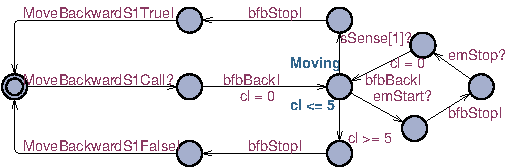
\includegraphics{MoveBackwardS1}
    \end{center}
    \caption{UPPAAL-automaat voor MoveBackwardS1. MoveBackwardS2, MoveForwardS1 en MoveForwardS2 zijn vrijwel identiek.}
    \label{fig:UPPAAL_MoveBackwardS}
    \end{figure}

    Figuur \ref{fig:UPPAAL_MoveBackwardS} is de automaat van
    MoveBackwardS1, de andere automaten lijken hier sterk op, behalve
    de richting waarin ze de band laten draaien en welke sensor ze
    controleren.

    Deze subroutine geeft de tweede lopende band opdracht in een
    bepaalde richting te gaan bewegen en komt dan in de Moving
    toestand. Vervolgens zijn er twee mogelijke uitkomsten:

    \begin{itemize}
        \item Als de lichtsensor iets waarneemt, wordt de band
        gestopt en een MoveBackwardS1True signaal aan het
        hoofdprogramma gegeven, dat aangeeft dat er inderdaad iets
        voor de sensor ligt.
        \item Als de lichtsensor na een bepaalde tijd nog niets
        gezien heeft, wordt de band gestopt en een
        MoveBackwardS1False signaal gegeven aan het hoofdprogramma
        om aan te geven dat er een time-out opgetreden is zonder dat
        de lichtsensor iets gedetecteerd heeft.
    \end{itemize}

    Een laaste mogelijkheid is nog dat er op de noodknop wordt
    gedrukt terwijl het programma in de Moving toestand is. In dit
    geval zal de band stoppen en als er weer op de noodknop wordt
    gedrukt begint de band opnieuw te lopen met de time-out weer
    teruggezet naar zijn begintoestand. In het assemblyprogramma zal
    deze time-out gewoon zijn waarde behouden.

    \subsection{Een wafer van de eerste lopende band pakken:
    LoadWafer}

    \begin{figure}
    \begin{center}
    
\includegraphics{LoadWafer}
    \end{center}
    \caption{UPPAAL-automaat voor LoadWafer.}
    \label{fig:UPPAAL_LoadWafer}
    \end{figure}

    Deze subroutine start beide lopende banden en komt dan in de
    Moving toestand. er zijn weer twee mogelijkheden om de moving
    toestand te verlaten:

    \begin{itemize}
        \item Als lichtsensor 1 iets waarneemt, ligt er blijkbaar
        een wafer klaar op band twee. Dan worden beide banden
        gestopt en krijgt het hoofdprogramma een LoadWaferTrue
        signaal om aan te geven dat er succesvol een wafer geladen
        is.
        \item Als er 10 seconden voorbij zijn en lichtsensor 1 heeft
        nog steeds niets waargenomen, lagen er blijkbaar geen wafers
        klaar op de eerste loopband. In dat geval worden beide
        loopbanden stilgezet en krijgt het hoofdprogramma een
        LoadWaferFalse signaal, om aan te geven dat er niet
        succesvol een wafer van de eerste band is gehaald.
    \end{itemize}

    Als er op de noodknop wordt gedrukt terwijl het programma in de
    Moving toestand is worden beide loopbanden gestopt. Als de
    noodknop dan weer wordt ingedrukt beginnen beide loopbanden weer
    en wordt begint de time-out weer in zijn begintoestand.\\

    Het is mogelijk dat er al een tweede wafer op de tweede lopende
    ban ligt voordat de lichtsensor de eerste detecteert. Volgens de
    opdrachtbeschrijving zouden de wafers echter met voldoende
    tussenruimte op de eerste band liggen op het moment dat er op de
    startknop wordt gedrukt en in dat geval levert dit geen
    problemen op.

    \section{Bediening deuren}

    Voor de bediening van de deuren zijn er vier subroutines, die
    verdeeld kunnen worden in twee groepen:

    \begin{itemize}
        \item Deuren openen
        \item Deuren sluiten
    \end{itemize}

    \subsection{Deuren openen: OpenDoor1, OpenDoor2}

    \begin{figure}
    \begin{center}
    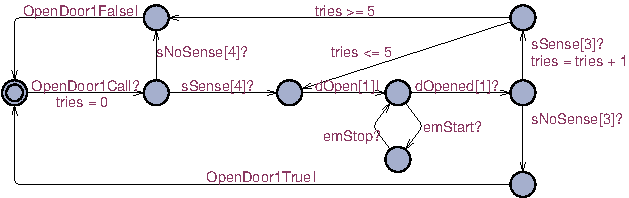
\includegraphics{OpenDoor1}
    \end{center}
    \caption{UPPAAL-automaat voor OpenDoor1. OpenDoor2 is vrijwel identiek.}
    \label{fig:UPPAAL_OpenDoor}
    \end{figure}

    In figuur \ref{fig:UPPAAL_OpenDoor} is de automaat van OpenDoor1
    afgebeeld, die van OpenDoor2 is hetzelfde, behalve dat die met andere
    sensoren en met de andere deur communiceert.\\

    Als deze routine wordt aangeroepen wordt eerst d.m.v. de
    druksensor bij deur 2 gekeken of deze deur wel echt dicht is.

    Als de deur open blijkt te zijn krijgt het hoofdprogramma een
    OpenDoor1False signaal, als de deur wel dicht is geeft deze
    routine opdracht om deur 1 te openen. Daarna controleert de
    subroutine of de deur ook echt opengegaan is d.m.v. de
    druksensor bij deur 1.

    Als de deur inderdaad open is krijgt het hoofdprogramma een
    OpenDoor1True signaal om aan te geven dat de deur succesvol
    opengemaakt is.

    Als de deur niet succesvol opengegaan is zal dit opnieuw
    geprobeerd worden, als de deur na vijf pogingen nog steeds niet
    open is krijgt het hoofdprogramma een OpenDoor1False signaal om
    aan te geven dat het openen van de deur mislukt is.


    \subsection{Deuren sluiten: CloseDoor1, CloseDoor2}

    \begin{figure}
    \begin{center}
    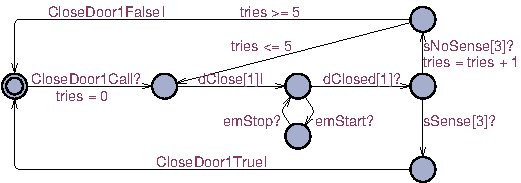
\includegraphics{CloseDoor1}
    \end{center}
    \caption{UPPAAL-automaat voor CloseDoor1. CloseDoor2 is vrijwel identiek.}
    \label{fig:UPPAAL_CloseDoor}
    \end{figure}

    Figuur \ref{fig:UPPAAL_CloseDoor} is de automaat van CloseDoor1, die van
    CloseDoor2 is identiek, behalve dat die met de andere deur en
    een andere sensor communiceert.\\

    In feite is deze subroutine ook identiek aan de
    OpenDoor-subroutines, behalve natuurlijk dat de deur hier gesloten
    wordt in plaats van geopend. Een tweede verschil is dat hier niet
    eerst wordt gecontroleerd in welke toestand de andere deur is,
    omdat het sluiten van een deur altijd is toegestaan.

    \section{Het belichten van een wafer: Burn}

    \begin{figure}
    \begin{center}
    
\includegraphics{Burn}
    \end{center}
    \caption{UPPAAL-automaat voor Burn.}
    \label{fig:UPPAAL_Burn}
    \end{figure}

    De subroutine hierboven handelt het belichten van een wafer af. In
    normale omstandigheden doorloopt deze subroutine alleen de
    onderste lus, die simpelweg de lamp inschakelt, twee seconden
    wacht, de lamp weer uitschakelt en dan een BurnTrue signaal
    geeft aan het hoofdprogramma om aan te geven dat het belichten
    goed gegaan is.

    Als echter de noodknop wordt ingedrukt terwijl de lamp aan is
    gaat de subroutine naar de bovenste lus, die in eerste instantie
    alleen maar de lamp uitschakelt. Als de noodknop weer wordt
    ingedrukt ten teken dat het systeem weer verder mag gaan zal
    de wafer naar de afvalbak vervoerd worden en vervolgens worden
    de deuren weer in de juiste stand gezet voor het verwerken van
    een volgende wafer, dus deur 2 dicht en deur 1 open. Vervolgens
    krijgt het hoofdprogramma een signaal BurnFalse om aan te geven
    dat het belichten mislukt is en dat begonnen kan worden met de
    verwerking van een eventuele volgende wafer. Merk op dat bij de
    afhandeling van deze noodstop gebruik wordt gemaakt van een
    aantal eerder in dit document behandelde subroutines.

    Als ��n van deze deuren niet goed open of dicht gaat komt de
    subroutine in de twee toestanden uiterst links en zal het
    programma crashen.

    \section{Verloren wafers afhandelen: HandleFalloff}

    \begin{figure}
    \begin{center}
    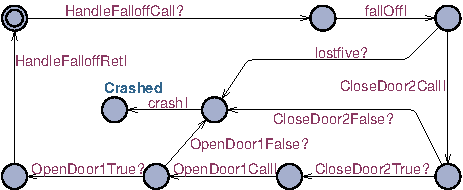
\includegraphics{HandleFalloff}
    \end{center}
    \caption{UPPAAL-automaat voor HandleFalloff.}
    \label{fig:UPPAAL_HandleFalloff}
    \end{figure}

    Als deze subroutine wordt aangeroepen wordt eerst een fallOff
    signaal gegeven aan de teller die het aantal verloren wafers
    bijhoudt. Als dan blijkt dat dit de vijfde wafer was die
    verloren ging gaat het programma naar de toestand in het midden
    en crasht het.

    Als er nog geen vijf wafers kwijtgeraakt zijn, zal deze
    subroutine zorgen dat de waferstepper klaar is om de volgende
    wafer af te handelen, dat wil zeggen: deur 2 wordt gesloten
    en deur 1 geopend. Als ��n van deze deuren niet goed open of
    dicht gaat, gaat de subroutine naar de toestanden in het midden
    en vervolgens crasht het programma.

    \section{Hulpautomaat om crashes te detecteren: ManageCrash}

    \begin{figure}
    \begin{center}
    
\includegraphics{ManageCrash}
    \end{center}
    \caption{UPPAAL-automaat voor ManageCrash}
    \label{fig:UPPAAL_ManageCrash}
    \end{figure}

    Zolang het programma draait zit deze automaat in de ``running''
    state. Zodra het programma ergens om een bepaalde reden crasht,
    dit kan zijn als een deur weigert te openen/sluiten of als er 5
    wafers kwijt zijn, wordt deze automaat in de ``crashed'' state
    gezet. Het nut van deze automaat is dat we gemakkelijk kunnen
    testen of het programma gecrasht is of niet, we hoeven nu
    namelijk niet alle afzonderlijke crash toestanden in de
    verschillende andere automaten te testen. 


    \chapter{Het hoofdprogramma}

    Het hoofdprogramma is gemodelleerd als een UPPAAL-template die
    de templates uit het vorige hoofdstuk aanstuurt op een zodanige
    manier dat het programma uiteindelijk doet wat het zou moeten
    doen: Het belichten van wafers en ze vervolgens in de daarvoor
    bestemde bak deponeren.\\


    \section{Het ontwerp}

    \begin{figure}
    \begin{center}
    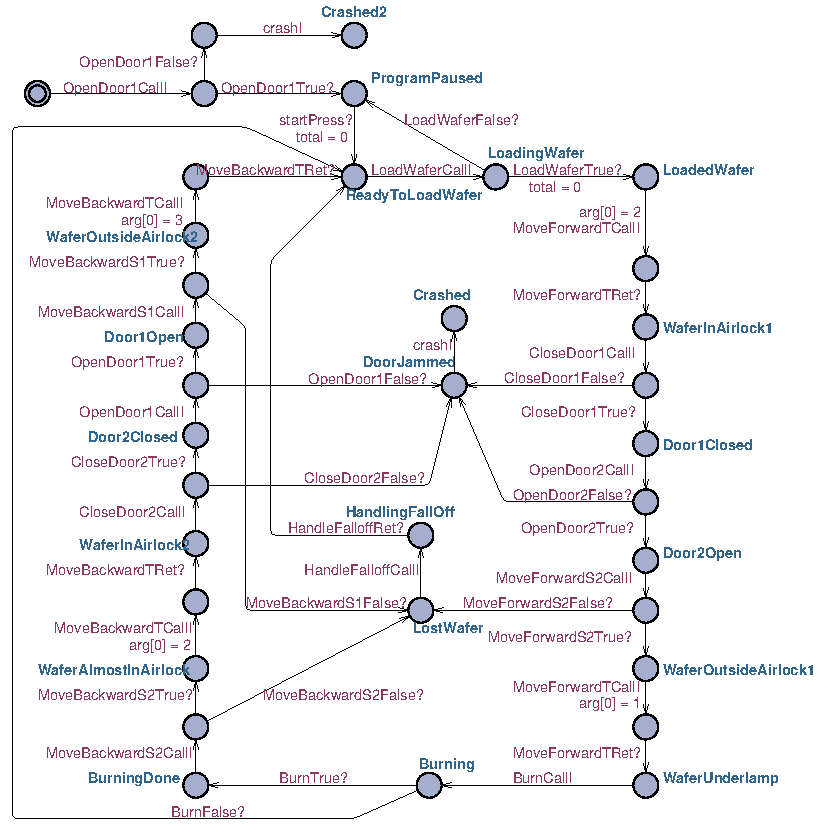
\includegraphics{Main}
    \end{center}
    \caption{UPPAAL-automaat van het hoofdprogramma.}
    \label{fig:UPPAAL_Main}
    \end{figure}

    Figuur \ref{fig:UPPAAL_Main} bevat de UPPAAL template voor het
    hoofdprogramma.

    Het eerste dat het programma doet is deur 1 openen, omdat in de
    begintoestand beide deuren gesloten zijn. Als dit mislukt crasht
    het programma onmiddellijk, anders gaat het naar de
    ProgramPaused toestand.\\

    In deze toestand wacht het programma totdat er op de startknop
    wordt gedrukt die aangeeft dat er wafers klaarliggen op de
    eerste band. Als deze knop wordt ingedrukt wordt LoadWafer
    aangeroepen. Dan wacht het programma totdat het een signaal
    terugkrijgt van deze subroutine.

    Als dit signaal LoadWaferFalse is, is er geen wafer van de eerste
    band gehaald en gaat het programma terug naar ProgramPaused,
    omdat er blijkbaar toch geen wafers klaarlagen.\\

    Als het programma een LoadWaferTrue signaal krijgt, ligt er een
    wafer klaar vlak voor de eerste deur van de luchtsluis en zal
    het programma deze wafer door de luchtsluis transporteren en
    onder de lamp leggen met behulp van de subroutines voor het
    bewegen van de lopende band en het openen en sluiten van deuren.
    Als dit alles goed gaat komt het programma in de WaferUnderLamp
    toestand.

    In dit traject kunnen echter enkele dingen misgaan. Er kan
    namelijk een deur weigeren open of dicht te gaan. In dat geval
    gaat het programma naar de DoorJammed toestand en vervolgens
    zal het crashen en in de Crashed toestand terechtkomen.

    Iets anders dat fout kan gaan is dat de wafer de tweede
    lichtsensor niet bereikt op het moment dat dat wel zou moeten.
    In dat geval wordt geconcludeerd dat de wafer verloren is gegaan
    en gaat het programma naar de LostWafer toestand. Daarna zal
    HandleFalloff aangeroepen worden. Als deze routine returnt is
    het systeem klaar om de volgende wafer te verwerken en gaat het
    programma naar ReadyToLoadWafer.\\

    Als alles echter goed gaat, ligt de wafer op dit moment onder de
    lamp en wordt er een aanroep gedaan naar Burn. Dit zorgt er in
    principe voor dat de wafer belicht wordt en dat het
    hoofdprogramma een BurnTrue signaal krijgt.

    Als er echter tijdens het belichten een noodstop plaatsvindt
    krijgt het hoofdprogramma een BurnFalse signaal. In dit geval is
    het systeem klaar voor het verwerken van de volgende wafer en
    gaat het programma dus terug naar ReadyToLoadWafer.\\

    Als alles goed gaat tijdens het belichten komt het programma in
    de toestand BurningDone. Vervolgens wordt de wafer door de
    luchtsluis naar de opvangbak getransporteerd. Dit proces en de
    zaken die hierbij mis kunnen gaan zijn vergelijkbaar met het
    naar binnen brengen van de wafer en zal hier ook niet verder
    toegelicht worden.\\

    Als de wafer in de bak ligt komt het systeem in toestand
    ReadyToLoadWafer en zal proberen de volgende wafer van de eerste
    band te halen. Als dit lukt begint het hele verhaal weer
    opnieuw, anders zijn blijkbaar alle wafers verwerkt en dan gaat
    het programma naar de ProgramPaused toestand, waar het wacht tot
    er op de startknop wordt gedrukt om aan te geven dat er weer
    wafers klaarliggen.


\end{document}
